\documentclass[10pt]{article}

\usepackage{spheric}
%%%TITLE
\title{Numerical modeling of 2D complex movement patterns to FSI problems using Smoothed Particle Hydrodynamics}
\date{}

%%AFFILIATIONS

\author[1,2]{Chen Zhuang}    
\author[1]{Dean Hu$^\dagger$}
\author[1,2]{Ting Long}
\author[1,2]{Gang Yang}

\affil[1]{State Key Laboratory of Advanced Design and Manufacturing for Vehicle Body, Hunan University, Changsha 410082, P. R. China}
\affil[2]{Key Laboratory of Advanced Design and Simulation Techniques for Special Equipment, Ministry of Education, Hunan University, Changsha 410082, P. R. China}

\affil[$\relax$]{\email{\dagger}{hudean@hnu.edu.cn}}


%%DOCUMENT
\begin{document}

\maketitle

%\SelectedTopics{}

%%PLEASE PUT YOUR ABSTRACT HERE
\begin{abstract}
Understanding dynamic behaviors of natural locomotion, such as aquatic animal swimming and
aerial animal flight, is very important for researchers and engineers who wish to develop robotics with good
locomotion capability. Aquatic and aerial locomotion generally have high efficiency, high maneuverability
and low noise with which no man-made robotics can compare. However, modeling and reproducing natural
locomotion using mesh-based numerical schemes, such as finite element method (FEM), finite volume
method (FVM) and finite difference method (FDM), are extremely challenged due to the highly mixed
patterns including translation, rotation, flexible motion and etc.

This paper presents a study based on weakly compressible smoothed particles hydrodynamics (WCSPH)
method, aiming at an available numerical modeling of two-dimensional (2D) complex movement patterns to
fluid-solid interaction (FSI) problems. The SPH scheme is first briefly recalled and discussed through its
formulations. Then a new technic based on dynamic boundary condition and designed to mimic the arbitrary
shapes with complex movement patterns is introduced. Two distinct test cases, including wedge water entry
and angularly reciprocating plate, are presented in order to validate this method. It has been found that there
is a general agreement between the simulation results and experimental data. Moreover, two novel cases
inspired by basilisk lizard locomotion \cite{glasheen1996hydrodynamic} and anguilliform swimming are conducted to show the capacity of
the computational model developed here for modeling the complex movement patterns.

\begin{figure}[!htb]
\centering
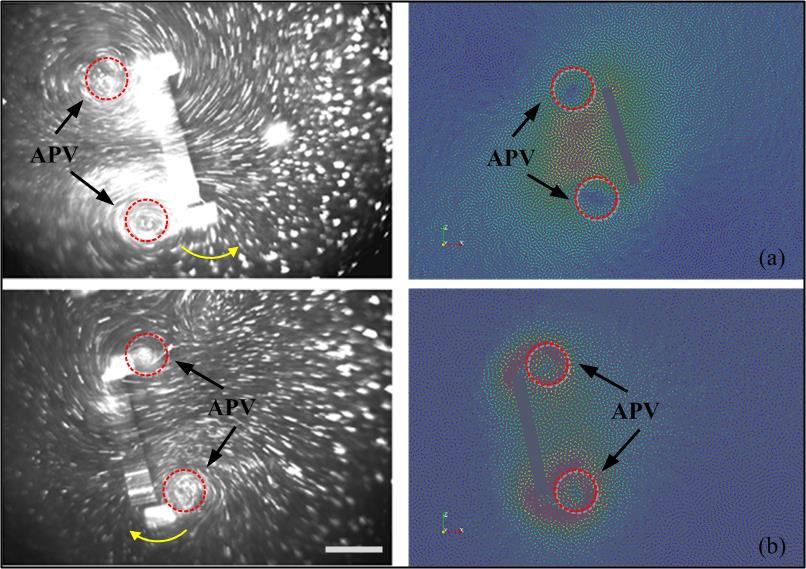
\includegraphics[width=0.7\textwidth]{42-1.png}
\caption{Comparison of flow structure around the angularly reciprocating plate between
experimental image by Lee \cite{lee2013wake} (left) and SPH (right). (a) APV at $\theta=10^\circ$; (b) APV at $\theta=5^\circ$. The round arrow indicates the instantaneous direction of flat-plate rotation.}\label{fig:}
\end{figure}

\end{abstract}


%%THE END OF ABSTRACT

\addbib

\end{document}
